\documentclass[12pt]{sftex/sftex}

\usepackage{graphicx, parskip}

\title{A emulação de consoles como \\ um artefato além da diversão}
\author{Caique R. Marques, Gustavo Zambonin, Douglas M. B. Martins}
\email{\{c.r.marques,gustavo.zambonin,marcelino.douglas\}@grad.ufsc.br}
\src{https://github.com/zambonin/pocket-higan}
\uniclass{Tópicos Especiais em Aplicações Tecnológicas III}
\classcode{UFSC-INE5450}

\begin{document}

\maketitle

\section{Prefácio}

Caracteriza-se como emulador todo hardware e software que habilita um computador
a comportar-se como outro sistema completamente diferente. Um emulador
tipicamente permite o uso de software programado para o sistema emulado, assim
expandindo a usabilidade do sistema original, e consequentemente, preservando
software para que seja conhecido no futuro. O desenvolvimento de tais construtos
mostra-se extremamente complicado, pois envolve o entendimento e simulação de
diversos componentes de um sistema que, por vezes, pode ser muito antigo ou
desconhecido.

Usualmente, um emulador é dividido em subsistemas: porções de código que
correspondem grosseiramente às partes do sistema alvo, como um simulador do
processador, um módulo de memória, vários dispositivos de entrada e saída, bem
como outros componentes: processadores de uso específico, periféricos e
eventuais barramentos necessários para a comunicação entre tais subsistemas.

Emuladores também podem estender as funcionalidades do sistema alvo; a aplicação
de \emph{aliasing} é extremamente comum para melhor qualidade dos gráficos;
latência diminuída no sistema de áudio; maior capacidade para armazenamento de
progresso; e por vezes é possível criar um sistema de comunicação entre
emuladores de modo a habilitar o \emph{multiplayer}.

Esse tipo específico de computação aplicada será discutida a partir de alguns
tópicos, enumerados abaixo, de modo a apresentar uma visão geral do estado da
vanguarda de emulação, seus benefícios e malefícios.

\section{Combate à obsolescência}

Um software está restrito a funcionar de acordo com as características dos
hardwares para o qual ele será destinado, portanto, nada pode garantir que
este mesmo software funcionará posteriormente, o que também poderá culminar com
o baixo uso e a raridade do software. Assim como qualquer registro histórico,
softwares também carregam informações de épocas nos quais eles foram criados e
para poder acessar seu conteúdo, são necessários o conhecimento e ferramentas da
época pertencente.

Uma das principais motivações dos emuladores é garantir a preservação do
software para o futuro, seja para usos pessoais, seja para estudos. Para
garantir a mesma experiência que o software oferecia para a época, é desejável
uma adaptação fiel da máquina em que ele foi designado originalmente, portanto,
será necessário uma simulação de tal hardware em outra máquina, que exige mais
desempenho e exige mais requisitos que o hardware original.

Entretanto, emuladores também podem ser considerados como uma forma ilegal de
usar o software, tendo em vista que os direitos para uso não estão sendo pagos;
assim, desenvolvedores criam métodos de proteção do software contra cópias não
autorizadas, sendo impossível usá-lo a não ser nas máquinas para o qual ele
foi designado. No SNES, o jogo Earthbound contém múltiplas verificações em
endereços de memória específicos que eram comumente alterados em cópias piratas;
caso tais modificações fossem encontradas, o número de encontros aleatórios com
inimigos aumenta drasticamente, e ao chegar em um certo ponto no final do jogo,
todo o progresso será deletado.

Recentemente tem existido um grande interesse por parte de empresas de jogos por
preservar seus lançamentos para o futuro e, também, por mostrar seus trabalhos
passados para a atual geração, neste caso, seja por plataformas que consigam
executá-las, seja por terceiros, trabalhando para a conversão para atuais
plataformas. A tendência dos relançamentos de jogos passados, por exemplo, é
melhorar a experiência e adaptar os requisitos de um jogo para os padrões
atuais.

\section{Visão técnica}

Emuladores essencialmente convertem informação binária escrita para funcionar em
um sistema para algo equivalente que possa executar em outro sistema desejável.
Essa conversão é geralmente feita traduzindo tais informações, na forma de
instruções, para equivalentes no sistema desejável. Entretanto, uma conversão
exata beira o impossível, e a adaptação do comportamento antigo para novos
sistemas mostra-se uma grande dificuldade na elaboração de software de emulação.
Conhecimento profundo sobre todas as partes do hardware a ser emulado é
necessário para que a comunicação entre estas seja programada corretamente

Tipicamente, consideram-se três formas de abordar a emulação no âmbito técnico:
a interpretação, e a tradução binária (ou recompilação, que por sua vez, pode
ser estática ou dinâmica).

\begin{itemize}

\item Na interpretação, a informação binária é lida e cada instrução é
decodificada e executada, toda vez que é encontrada. Geralmente, este método é
o mais fácil de ser implementado (e consequentemente, sincronizado, depurado
e portado), mas também o mais lento. O algoritmo genérico para este tipo de
emulação pode ser resumido como:

\begin{verbatim}
faça
    busque a próxima instrução da memória emulada
    execute a instrução
    verifique quaisquer interrupções
enquanto ( CPU está rodando )
\end{verbatim}

\item A tradução binária dinâmica elimina o laço supracitado traduzindo pequenas
sequências de código (como um bloco básico) e armazenando tais informações para
que possam ser referenciadas em um momento posterior. A ideia por trás desta
abordagem é diminuir o tempo de tradução, que é um grande gargalo para o
desempenho do software, e referenciar código armazenado o máximo possível. Este
método é o mais comum por conseguir lidar com qualquer tipo de código, incluindo
porções que podem mudar ao longo da execução, mas a dificuldade de implementar a
sincronização entre as operações aumenta exponencialmente. Um emulador conhecido
que utiliza a compilação JIT\footnote{\emph{just-in-time}, ou seja, compilação
feita durante a execução de um programa. Pode empregar a recompilação dinâmica
como um método de otimização.} é o \href{https://dolphin-emu.org/}{Dolphin}.

\item A tradução binária estática funciona de maneira similar à dinâmica,
salvando o resultado em disco ou na memória, para referência posterior. Porém,
esta técnica usualmente falha quando o código pode ser modificado no meio da
execução, já que não existe tradução disponível para as novas informações.
Assim, este método é geralmente combinado com um tradutor binário dinâmico ou um
interpretador.

\end{itemize}

\section{Desempenho}

O emulador \texttt{\href{http://byuu.org/emulation/higan/}{higan} v095}, obtido
de maneira usual pelo gerenciador de pacotes do sistema operacional Arch Linux,
foi testado com o jogo Super Mario World em três sistemas de especificações
variadas: um Raspberry Pi 1 Model B (Broadcom BCM2835), para representar a
performance no âmbito portátil; um laptop de desempenho médio (Intel Core
i5--4210U @ 1.70GHz, GeForce GT 740M); e um computador de mesa (Intel Core
i3--2100 @ 3.10GHz, Intel HD Graphics 2000).

Os resultados foram obtidos a partir da execução do emulador com o
\emph{backend} de vídeo SDL\footnote{Simple DirectMedia Layer ---
\url{https://www.libsdl.org/}}, e são mensurados em FPS\footnote{\emph{frames
per second}, a frequência em que um dispositivo de processamento de imagens
produz consecutivas imagens, chamadas de quadros.}. Os núcleos otimizados para
precisão (\texttt{accuracy}), desempenho (\texttt{performance}) e ``meio-
termo'' (\texttt{balanced}) foram unificados em versões mais novas do emulador
em virtude da vasta complexidade necessária para mantê-los; assim, resultados
com tais versões podem ser diferentes.

\begin{table}[ht]
\centering
\begin{tabular}{lccccccccc}
& \multicolumn{3}{c}{BCM2835} & \multicolumn{3}{c}{Core i5}
    & \multicolumn{3}{c}{Core i3} \\
& min & med & max & min & med & max & min & med & max \\
\texttt{higan-accuracy}
    & 1   & 1   & 2   & 49  & 56  & 60  & 56  & 58  & 59  \\
\texttt{higan-balanced}
    & 2   & 2   & 3   & 60  & 60  & 61  & 169 & 180 & 189 \\
\texttt{higan-performance}
    & 2   & 2   & 3   & 59  & 60  & 61  & 293 & 302 & 311 \\
\end{tabular}
\caption{Desempenho de vários sistemas rodando \texttt{higan}. Valores médios
são aproximados para baixo.}
\end{table}

Emuladores requerem hardware mais maduro do que o sistema alvo; os recursos
necessários para simular um sistema completo em software são extraordinários,
como é possível verificar nos resultados acima. O console SNES funcionava, a uma
taxa de quadros de no mínimo 30 FPS, com o processador Ricoh 5A22 operando a
3.58 MHz, enquanto o BCM2835 presente no Raspberry Pi testado contém um
ARM1176JZF-S com frequência de 700 MHz --- cerca de duzentas vezes maior.

Porém, a precisão obtida com esta grande perda de desempenho é notável em alguns
casos especiais, caso a emulação seja concebida corretamente em software. Por
exemplo, diferentemente da maioria dos emuladores, \texttt{higan} renderiza a
S-PPU\footnote{\emph{SNES Picture Processing Unit}} pixel por pixel, enquanto a
estratégia comum baseia-se em renderizar a \emph{scanline}\footnote{linhas de
uma imagem que é composta por pixels, como em um monitor CRT.} inteira a partir
de um ponto fixo. A emulação torna-se 40\% mais lenta~\cite{emustate} com esta
tática, porém faz uma grande diferença no jogo Air Strike Patrol, que utiliza
pedidos de interrupção (IRQs) especialmente sincronizados de modo a ajustar o
registrador de brilho da tela, para criar um sombreado translúcido embaixo do
avião controlado pelo jogador.

\begin{figure}[ht]
\centering
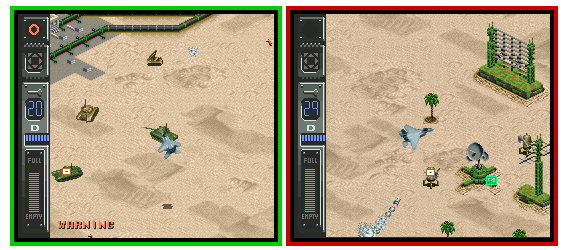
\includegraphics[scale=0.70]{images/airforce}
\caption{À esquerda, a sombra do avião é corretamente emulada, desenhando a
\emph{scanline} com valores de brilho heterogêneos. À direita, a emulação
incorreta: não existe uma referência para acertar inimigos, aumentando a
dificuldade do jogo. Imagem retirada de~\cite{accpower}.}
\end{figure}

\section{Segundo a lei}

As leis variam dependendo do país, mas no geral, o uso de emuladores é taxado
como ilegal por infringir direitos autorais.  No Brasil, de acordo com o Inciso
I do Art. 6º de~\cite{lei9609}, é legal o usuário copiar

\begin{quote}
$(\ldots)$ um só exemplar, de cópia legitimamente adquirida, desde que se
destine à cópia de salvaguarda ou armazenamento eletrônico, hipótese em que
o exemplar original servirá de salvaguarda.
\end{quote}

ou seja, o usuário só poderá ter uma (e apenas uma) ROM\footnote{\emph{Read-Only
Memory}, abreviação comum para referenciar o arquivo copiado da mídia original.}
de um jogo, se ele já tiver a cópia original. Ainda, a ROM serve apenas para
fins de armazenamento e seu uso é apenas válido caso a cópia original adquirida
esteja indisponível.

Na questão de domínio público, o § 2º do Art. 2º de~\cite{lei9609} descreve que

\begin{quote}
Fica assegurada a tutela dos direitos relativos a programa de computador pelo
prazo de cinquenta anos, contados a partir de 1º de janeiro do ano subsequente
ao da sua publicação ou, na ausência desta, da sua criação.
\end{quote}

Portanto, um programa pode entrar em domínio público apenas cinquenta anos após
a publicação (ou a criação, caso não tenha sido publicado), antes disto, os
direitos permanecem a quem os detêm, mesmo que não haja uso ativo do programa.
Assim como obras artísticas, o período para que para que um programa entre em
domínio público varia dependendo do país. Nos Estados Unidos, por exemplo, tais
obras só são configuradas como domínio público após setenta e cinco anos desde a
data de publicação.

Para contornar o uso de emuladores e disponibilizar jogos que já não são
acessíveis em mídia original, algumas empresas publicam coletâneas ou
relançamentos dos jogos para as mais variadas plataformas por preços mais
reduzidos; porém, em alguns casos, tais emulações são feitas de modo divergente
ao funcionamento original, assim danificando a preservação do software.

\section{Epílogo}
O principal problema enfrentado pelos emuladores é garantir a fidelidade do
hardware em que ele quer simular, exigindo conhecimento profundo deste
hardware, mesmo assim, a sua simulação nunca chega a total fidelidade, visto as
capacidades das máquinas de conseguir emular uma outra arquitetura em si, mas
consegue apresentar o proposito em que o hardware original, juntamente com
softwares, quiseram passar.

O uso ainda é assunto de debate, apesar de emuladores serem taxados como
ilegais, por também ser um meio de usufruir de tecnologias sem pagar os
direitos autorais.  No entanto, até mesmo no mercado, emuladores são usados
para fins de estudo, como foi o caso do programador e game designer Yuji Naka,
conhecido como um dos criadores do personagem de videogames Sonic the Hedgehog,
que trabalhou no desenvolvimento de um emulador de Famicom (conhecido como
Nintendo Entertainment System no ocidente) para o Mega Drive, que era
concorrente do console na época, no final dos anos 1980, o resultado, segundo
ele, não foi satisfatório --- isto é um dos primeiros registros de emuladores
entre consoles de videogame.

Emuladores são ferramentas de estudo, com eles é possível simular um hardware e
verificar softwares que até então não poderiam ser analisados, seja por
indisponibilidade, seja por questões práticas específicas. Emuladores são
cápsulas do tempo, possibilitam o averiguamento de tecnologias mais antigas,
trazendo informações e o conhecimento passados que são fundamentais para o
estudo da história humana.

\bibliography{ine5450}
\bibliographystyle{plain}

\end{document}
